\documentclass[a4paper, 12pt]{article}
\usepackage{graphicx}
\usepackage{xcolor}
\usepackage[margin=1cm]{geometry}
\usepackage[normalem]{ulem}
\usepackage{multicol}
\usepackage{enumitem}

\begin{document}
\thispagestyle{empty} % no page number

\begin{figure}[!ht]
    \centering
    
\includegraphics[width=\textwidth]{head}
\vspace{1em}
    {\color{black}\rule{\textwidth}{0.8pt}}
\end{figure}
%%%%%%%%%%%%%%%%%%%%%%%%%%%%%%%%%%%%%%%%%%%
\hspace{-0.35cm} {\Large \bfseries Errata \small (last updated: 2026-10-12)}

\begin{itemize}[leftmargin=*]
	\item[] Thesis. p.63. \textbf{Knowledge gap.} Andersson et al. [\sout{90} 16]
	\item[] Thesis. p.64. \textbf{Table 7.1.} Andersson et al. [\sout{90} 16]
	\item[] Thesis. p.97. \textbf{References 60} should be corrected to the following:
	Bower H, Björkholm M, Dickman PW, Höglund Martin, Lambert PC, Andersson TML. Life Expectancy of Patients With Chronic Myeloid Leukemia Approaches the Life Expectancy of the General Population. Journal of Clinical Oncology. 2016;34(24):2851-7.
	\item[] Study II. p.300. \textbf{2.1.2 Transition 2: Modeling the Mortality Rate of Progression-Free to Death.} "Note that model fitting for $H_{2}(t, t+a, t+c)$ uses the \sout{all-cause mortality rates} expected mortality rates $h^{*}_{2}(t+a, t+c)$ for the event times and does not require \sout{all-cause cumulative mortality rates} cumulative expected mortality rates $H^{*}_{2}(t+a, t+c)$, as minus $H^{*}_{2}(t+a, t+c)$ is a constant term in the log-likelihood."
	
\item[] \begin{multicols}{3}
\begin{minipage}{\linewidth}
Study IV Manuscript. p.14. \textbf{Table 3 (Continued).} \par
\centering
\vspace{0.53cm}
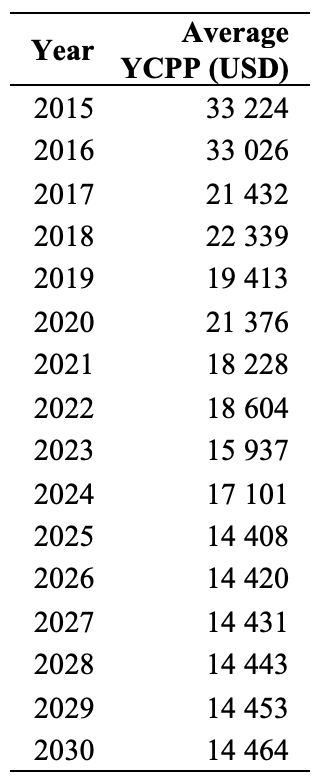
\includegraphics[width=0.65\linewidth]{Table3.png}%
\hspace{0.5cm}%
\end{minipage}

\begin{minipage}{\linewidth}
Study IV Supplementary Materials. p.22. \textbf{Table S5 (Continued).} \par
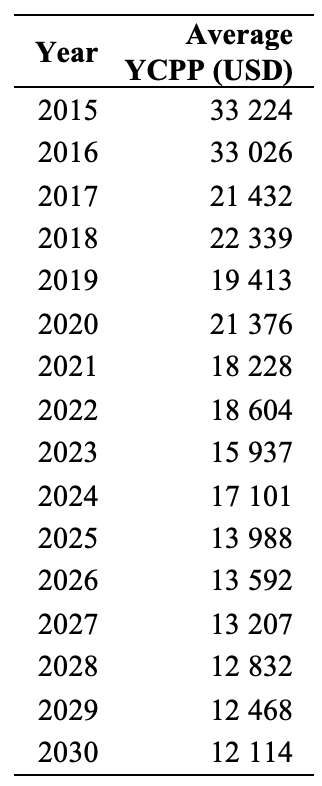
\includegraphics[width=0.65\linewidth]{TableS5.png}
\centering
\end{minipage}

\begin{minipage}{\linewidth}
Study IV Supplementary Materials. p.24. \textbf{Table S6 (Continued).} \par
\vspace{-0.01cm}
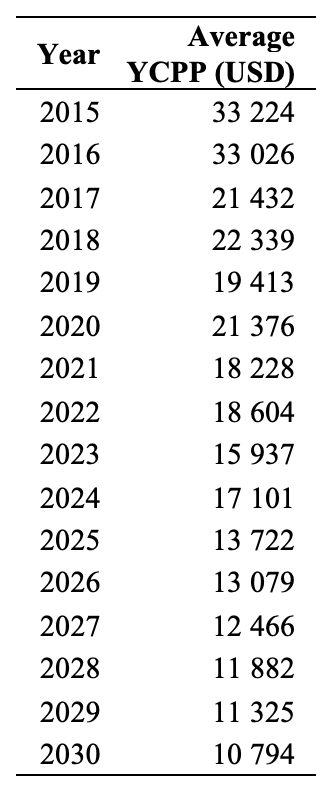
\includegraphics[width=0.65\linewidth]{TableS6.png}
\centering
\end{minipage}
\end{multicols}

\end{itemize}

\newpage
\thispagestyle{empty} % no page number

Study IV Supplementary Materials. p.13. \textbf{Figure S5.}

\begin{figure}[ht]
\centering
	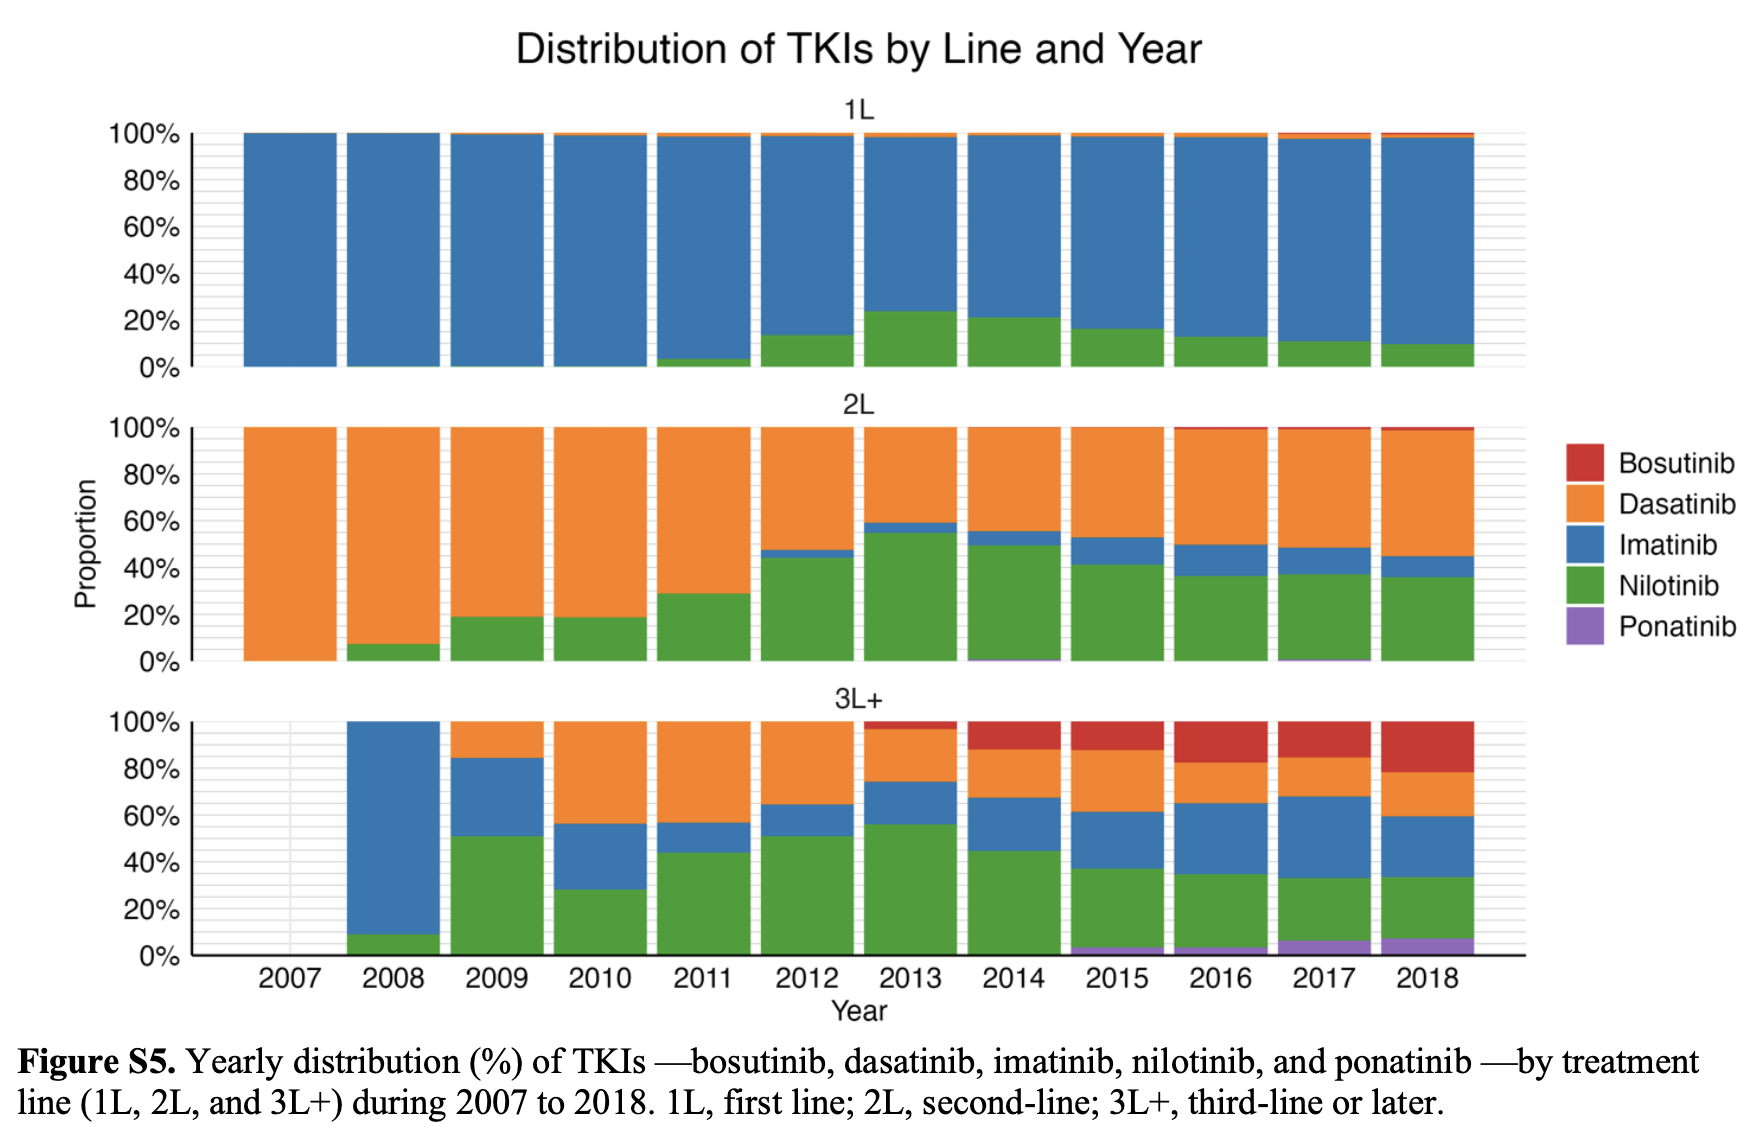
\includegraphics[width=1\linewidth]{FigureS5.png}%
\end{figure} 

\end{document}
